\section{Pellsche Gleichungen}\label{kapitel:Pell}
\emph{Pellsche Gleichungen}, fälschlicherweise benannt nach John Pell (1611--1685) sind Diophantische Gleichungen der Form $x^2-dy^2=k$. Hierin ist $k$ eine ganze Zahl und $d$ eine positive ganze Zahl, die keine Quadratzahl ist.\footnote{Wäre $d=a^2$ eine Quadratzahl, ließe sich die Gleichung zu $(x-ay)(x+ay)=k$ faktorisieren und aus der Primfaktorzerlegung von $k$ ließen sich alle Lösungen ablesen. Dieser Fall ist also trivial.} Gesucht sind alle ganzzahligen Lösungspaare $(x,y)$.

Zahlreiche Olympiade-Aufgaben lassen sich, nach geschickter Vereinfachung, auf Pellsche Gleichungen zurückführen. Deswegen ist es wichtig, dass ihr wisst, wie sich solche Gleichungen lösen lassen. Unser Ziel in diesem Kapitel ist, den folgenden, alles andere als offensichtlichen Satz zu beweisen:
\begin{satzmitnamen}[Lösbarkeit der Pellschen Gleichung]
	Sei $k$ eine ganze Zahl und sei $d$ eine positive ganze Zahl, die keine Quadratzahl ist.
	\begin{enumerate}[label={$(\alph*)$},ref={$(\alph*)$}]
		\item Die Pellsche Gleichung $x^2-dy^2=1$ hat stets unendlich viele ganzzahlige Lösungen $(x,y)$.
		\item Wenn die Pellsche Gleichung $x^2-dy^2=k$ eine ganzzahlige Lösung $(x,y)$ hat, dann hat sie unendlich viele ganzzahlige Lösungen.
	\end{enumerate}
\end{satzmitnamen}
Der Beweis bedarf einiger Vorbereitungen.

\subsection*{Die Norm in $\boldsymbol{\mathbb Z[\sqrt{d}]}$}
Wenn $d$ eine Quadratzahl wäre, könnten wir den Ausdruck $x^2-dy^2$ gemäß der dritten binomischen Formel in zwei ganzzahlige Faktoren zerlegen. Die entscheidende Idee zum Lösen Pellscher Gleichungen besteht darin, die gleiche Faktorisierung auch dann zu betrachten, wenn $d$ keine Quadratzahl ist: Die Gleichungen $x^2-dy^2=1$ und $x^2-dy^2=k$ werden dann zu
\begin{equation*}
	\parens*{x+y\sqrt{d}}\parens*{x-y\sqrt{d}}=1\quad\text{und}\quad \parens*{x+y\sqrt{d}}\parens*{x-y\sqrt{d}}=k\,.
\end{equation*}
Freilich sind die Faktoren keine ganzen Zahlen mehr. Wir müssen also anstelle von $\mathbb Z$ die Menge $\braces{a+b\sqrt{d}\ |\ a,b\in\mathbb Z}$ betrachten. Diese Menge wollen wir mit $\mathbb Z[\sqrt{d}]$ bezeichnen. 

Wir überlegen uns zuerst, dass die Darstellung $z=a+b\sqrt{d}$ mit $a,b\in \mathbb Z$ eindeutig ist. Wären nämlich $a_1+b_1\sqrt{d}=a_2+b_2\sqrt{d}$ zwei verschiedene Darstellungen, dann muss $b_1\neq b_2$ sein, denn aus $b_1=b_2$ folgt auch $a_1=a_2$. Durch Umformen folgt nun $\sqrt{d}=(a_1-a_2)/(b_2-b_1)$. Somit wäre $\sqrt{d}$ wäre eine rationale Zahl, was aber nicht sein kann, denn $d$ ist keine Quadratzahl.

Zahlen aus $\mathbb Z[\sqrt{d}]$ können wir addieren, subtrahieren und multiplizieren und das Ergebnis wird stets wieder in $\mathbb Z[\sqrt{d}]$ liegen. Außerdem lassen sich Zahlen \emph{konjugieren}: Zu einer Zahl $z=x+y\sqrt{d}\in\mathbb Z[\sqrt{d}]$ definieren wir die \emph{zu $z$ konjugierte Zahl} als $\overline{z}\coloneqq x-y\sqrt{d}$. Es lässt sich unmittelbar nachprüfen, dass für die Konjugation die Rechenregeln
\begin{equation*}
	\overline{\overline{z}}=z\,,\quad \overline{z_1\pm z_2}=\overline {z_1}\pm \overline{z_2}\quad\text{und}\quad \overline{z_1\cdot z_2}=\overline{z_1}\cdot\overline{z_2}
\end{equation*}
für alle $z,z_1,z_2\in\mathbb Z[\sqrt{d}]$ gelten. 

Wenn euch $\mathbb Z[\sqrt{d}]$ jetzt an die komplexen Zahlen erinnert, dann liegt ihr vollkommen richtig. Die komplexen Zahlen $\mathbb C$ entstehen aus den reellen Zahlen, indem wir eine Lösung der in $\mathbb R$ nicht lösbaren quadratischen Gleichung $X^2+1=0$ hinzufügen.\footnote{Statt \emph{hinzufügen} wird in der Mathematik meistens \emph{adjungieren} gesagt.} Ebenso entsteht $\mathbb Z[\sqrt{d}]$ aus $\mathbb Z$, indem wir eine Lösung der in $\mathbb Z$ nicht lösbaren quadratischen Gleichung $X^2-d=0$ hinzufügen. Für komplexe Zahlen gibt es den \emph{Betrag}, der duch $\abs{z}^2=z\cdot \overline{z}$ definiert ist. Analog definieren wir für $z=x+y\sqrt{d}\in\mathbb Z[\sqrt{d}]$ die \emph{Norm von $z$} durch
\begin{equation*}
	N(z)=z\cdot \overline z=\left(x+y\sqrt{d}\right)\left(x-y\sqrt{d}\right)=x^2-dy^2\,.
\end{equation*}
Genau wie der komplexe Betrag verträgt sich auch die Norm mit Multiplikation, das heißt es gilt $N(z_1z_2)=N(z_1)N(z_2)$ für alle $z_1,z_2\in\mathbb Z[\sqrt{d}]$.

Die Pellschen Gleichungen $x^2-dy^2=1$ und $x^2-dy^2=k$ können wir jetzt wie folgt umschreiben:
\begin{equation*}
	N\parens*{x+y\sqrt{d}}=1\quad\text{und}\quad N\parens*{x+y\sqrt{d}}=k\,.
\end{equation*}
Statt nach Paaren $(x,y)$ von ganzen Zahlen mit $x^2-dy^2=1$ können wir also äquivalenterweise nach Zahlen $z\in\mathbb Z[\sqrt{d}]$ mit $N(z)=1$ suchen. Offenbar gilt $N(1)=N(-1)=1$, korrespondierend zu den beiden trivialen Lösungen $(x,y)=(1,0)$ und $(x,y)=(-1,0)$ von $x^2-dy^2=1$. Wenn $N(z)=1$, dann gilt auch $N(\overline{z})=1$, $N(-z)=1$ und $N(-\overline{z})=1$. Das korrespondiert zu der Beobachtung, dass mit $(x,y)$ auch $(\pm x,\pm y)$ Lösungen der Gleichung $x^2-dy^2=1$ sind.

Diese Beobachtung erlaubt uns, den Zahlenraum, in dem wir nach Lösungen von $N(z)=1$ suchen, ein wenig einzuschränken. Indem wir $z$ gegebenenfalls durch $-z$ ersetzen, dürfen wir nämlich $z>0$ annehmen. Indem wir $z$ gegebenenfalls durch $\overline{z}=\frac 1z$ ersetzen (denn $z\cdot \overline{z}=N(z)=1$), dürfen wir ferner $z\geqslant 1$ annehmen. Wir dürfen uns somit auf Lösungen von $N(z)=1$ mit $z\geqslant 1$ beschränken. Das korrespondiert zu der Einschränkung $x\geqslant 1$, $y\geqslant 0$.

Wir können jetzt eine Verschärfung des gewünschten Satzes formulieren.
\begin{satzmitnamen}[Lösbarkeit der Pellschen Gleichung \textmd{(verbesserte Version)}]
	Sei $k$ eine ganze Zahl und $d$ eine natürliche Zahl, die keine Quadratzahl ist.
	\begin{enumerate}
		\item Die Gleichung $N(z)=1$ in $\mathbb Z[\sqrt{d}]$ hat unendlich viele Lösungen. Unter allen Lösungen mit $z>1$ gibt es eine minimale Lösung $z_0$, die sogenannte Fundamentallösung. Alle weiteren Lösungen $z$ sind durch $z=\pm z_0^n$ mit $n\in\mathbb Z$ gegeben.\label{behauptung:PellscheGleichung=1}
		\item Wenn die Gleichung $N(z)=k$ in $\mathbb Z[\sqrt{d}]$ eine Lösung $z=u$ hat, dann lassen sich unendlich viele weitere Lösungen durch $z=\pm u\cdot z_0^n$ finden, wobei~$z_0$ die Fundamentallösung aus~\ref{behauptung:PellscheGleichung=1} ist. Im Fall $k=-1$ sind alle Lösungen von dieser Form \embrace{für allgemeines $k$ muss das jedoch nicht der Fall sein}.\label{behauptung:PellscheGleichung=k}
	\end{enumerate}
\end{satzmitnamen}
\begin{proof}
	Der komplizierteste Teil des Beweises besteht darin, zu zeigen, dass eine nichttriviale Lösung $z\neq \pm1$ der Gleichung $N(z)=1$ existiert. Diesen Beweis werden wir im nächsten Unterabschnitt führen. Wir werden einstweilen die übrigen Aussagen beweisen.
	
	Aus dem obigen Argument folgt: Wenn eine Lösung mit $z\neq \pm 1$ existiert, dann existiert auch eine Lösung mit $z>1$. Schreibe $z=x+y\sqrt{d}$ mit $x> 1$, $y> 0$. Wenn $z_0=x_0+y_0\sqrt{d}$ eine weitere Lösung mit $z\geqslant z_0>1$ ist, dann müssen die Ungleichungen $x\geqslant x_0> 1$ und $y\geqslant y_0> 0$ gelten (eine von beiden Ungleichungen muss auf jeden Fall gelten, sonst wäre nicht $z\geqslant z_0$; die andere folgt dann automatisch aus $x^2-dy^2=1=x_0^2-dy_0^2$). Also gibt es nur endlich viele Lösungen $z_0$ mit $z\geqslant z_0>1$. Insbesondere muss tatsächlich eine minimale Lösung $z_0$ existieren.
	
	Jede weitere Lösung mit $z> 0$ muss dann von der Form $z=z_0^n$ für eine ganze Zahl $n$ sein. Ansonsten gäbe es nämlich ein $n$ mit $z_0^{n}<z<z_0^{n+1}$. Dann ist $1<z\cdot z_0^{-n}<z_0$. Wegen $z_0\cdot \overline{z_0}=N(z_0)=1$ ist $z\cdot z_0^{-n}=z\cdot \overline{z_0}^{n}$ ein Element von $\mathbb Z[\sqrt{d}]$. Schließlich gilt
	\begin{equation*}
		N\parens*{z\cdot z_0^{-n}}=N(z)\cdot N(z_0)^{-n}=1\cdot 1^{-n}=1
	\end{equation*}
	Dann widerspricht $z\cdot z_0^{-n}$ aber der Minimalität von $z_0$. Unsere Annahme war somit falsch und $z$ muss tatsächlich von der Form $z=z_0^n$ sein. Analog muss jede Lösung mit $z<0$ von der Form $z=-z_0^n$ sein. Ansonsten gäbe es ein $n$ mit $-z_0^{n+1}<z<-z_0^n$. Analog zu oben würde dann $-z\cdot z_0^n$ der Minimalität von $z_0$ widersprechen. Damit ist~\ref{behauptung:PellscheGleichung=1} gezeigt (bis auf die Existenz einer nichttrivialen Lösung).
	
	Für~\ref{behauptung:PellscheGleichung=k} benutzen wir, dass die Norm multiplikativ ist, um $N(\pm u\cdot z_0^n)=N(\pm 1)\cdot N(u)\cdot N(z_0)^n=1\cdot k\cdot 1^n=k$, zu rechnen. Im Fall~$k=-1$ gilt $u\cdot \overline{u}=N(u)=-1$. Also können wir in $\mathbb Z[\sqrt{d}]$ durch $u$ dividieren, denn Division durch $u$ ist das Gleiche wie Multiplikation mit $\frac 1u=-\overline{u}$. Wenn~$z$ eine Lösung von $N(z)=-1$ ist, die nicht von der Form $\pm u\cdot z_0^n$ ist, dann wäre $z/u$ nicht von der Form $\pm z_0^n$. Es gilt aber $-1=N(z)=N(z/u\cdot u)=N(z/u)\cdot N(u)=-N(z/u)$, also $N(z/u)=1$. Damit würde $z/u$ der in \ref{behauptung:PellscheGleichung=1} bewiesenen Klassifikation aller Elemente von Norm~$1$ widersprechen.
\end{proof}

Wenn ihr Lösungen der Gleichung $N(z)=1$ mit $z\in\mathbb Z[\sqrt{d}]$ zurück in Lösungen der Pellschen Gleichung $x^2-dy^2=1$ übersetzen wollt, könnt ihr die Bedingung $z=\pm z_0^n$ folgendermaßen umformulieren: Wenn die Pellsche Gleichung $x^2-dy^2$ die minimale nichttriviale Lösung $(x,y)=(x_0,y_0)$ mit $x_0>1$ und $y_0>0$ besitzt, dann ist jede weitere Lösung $(x,y)$ mit $x>1$ und $y>0$ durch die folgende Rekursion gegeben:
\begin{equation*}
	x_{n+1}=x_0x_n+dy_0y_n\quad\text{und}\quad y_{n+1}=x_0y_n+x_ny_0
\end{equation*}
(die Gleichungen sind äquivalent zu $x_{n+1}+y_{n+1}\sqrt{d}=(x_0+y_0\sqrt{d})(x_n+y_n\sqrt{d})$). Statt dieser Rekursion solltet ihr euch aber lieber die Gleichung $z=\pm z_0^n$ merken -- das ist wesentlich einfacher und erklärt, woher die Rekursion wirklich kommt.

\subsection*{Existenz einer nichttrivialen Lösung}
Wir machen uns jetzt daran, den schwierigsten Schritt im Beweis der Lösbarkeit der Pellschen Gleichung durchzuführen und eine nichttriviale Lösung zu konstruieren. Die zentrale Idee ist hierbei folgende: Wenn $(x,y)$ die Pellsche Gleichung $x^2-dy^2=1$ löst und $x>1$, $y>0$ gilt, dann ist $x^2\approx dy^2$, also $x/y\approx \sqrt{d}$. Mit anderen Worten: $x/y$ ist eine \emph{rationale Approximation} der irrationalen Zahl $\sqrt{d}$. Um die Pellsche Gleichung zu lösen, gehen wir umgekehrt vor. Wir konstruieren zuerst sehr genaue rationale Approximationen der irrationalen Zahl $\sqrt{d}$ und beweisen dann, dass wir dadurch (manchmal) Lösungen der Pellschen Gleichung bekommen.

Um genaue Approximationen von irrationalen Zahlen zu konstruieren, benutzen wir das folgende Lemma, das auf Gustav Lejeune Dirichlet (1805--1859) zurückgeht.

\begin{satzmitnamen}[Dirichletscher Approximationssatz]
	Sei $\alpha$ eine irrationale reelle Zahl. Dann gibt es unendlich viele Paare $(p,q)$ von ganzen Zahlen mit $q>0$ und
	\begin{equation*}
		\abs*{\alpha-\frac{p}{q}}<\frac{1}{q^2}\;.
	\end{equation*}
\end{satzmitnamen}
Intuitiv besagt der Dirichletsche Approximationssatz besagt, dass wir $\alpha$ \enquote{effizient} (relativ zum Nenner) durch rationale Zahlen annähern können.

\begin{wrapfigure}{r}{0.2\textwidth}
	\centering\vspace{-0.7cm}
	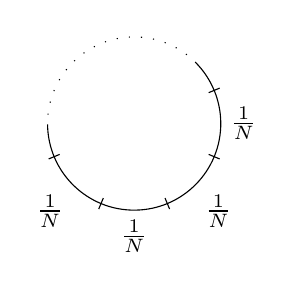
\begin{tikzpicture}[x=0.55cm,y=0.55cm, rotate=22.5]
		%\draw(0,0) circle (2);
		\draw[loosely dotted] (22:2) arc (22:158:2);
		\draw (158:2) arc (158:382:2);
		\draw (0:2) ++ (0:0.5ex) to ++(0:-1ex);
		\draw (315:2) ++ (315:0.5ex) to ++(315:-1ex);
		\draw (270:2) ++ (270:0.5ex) to ++(270:-1ex);
		\draw (225:2) ++ (225:0.5ex) to ++(225:-1ex);
		\draw (180:2) ++ (180:0.5ex) to ++(180:-1ex);
		\node[right] at (337.5:2) {$\frac{1}{N}$};
		\node[below right] at (292.5:2) {$\frac{1}{N}$};
		\node[below] at (247.5:2) {$\frac{1}{N}$};
		\node[below left] at (202.5:2) {$\frac{1}{N}$};
	\end{tikzpicture}
	\vspace{-0.5cm}
\end{wrapfigure}
\begin{proof}
	Wir stellen uns einen Kreis vom mit Umfang $1$ vor, um den wir mit Schritten der Länge $\alpha$ herumlaufen. Wähle eine positive ganze Zahl $N$. Wir unterteilen den Kreis in $N$ Abschnitte der Länge $\frac1N$ (wobei die \glqq Grenzen\grqq\ zwischen zwei Abschnitten immer zu demjenigen Abschnitt dazuzählen sollen, der -- gegen den Uhrzeigersinn betrachtet -- vor dem anderen Abschnitt liegt). Wenn wir den Anfangspunkt als nullten Schritt mitzählen, müssen wir gemäß dem Schubfachprinzip nach $N$ Schritten zweimal im gleichen Abschnitt gelandet sein. Es gibt also natürliche Zahlen $0\leqslant m<n\leqslant N$, sodass die Endpunkte nach $m\alpha$ und $n\alpha$ Umläufen um den Kreis weniger als $\frac 1N$ auseinanderliegen, das heißt wir finden eine ganze Zahl $p$ mit 
	\begin{equation*}
		\abs*{n\alpha-m\alpha-p}<\frac1N\,.
	\end{equation*}
	Mit $q=n-m$ gilt dann $q\leqslant N$ und damit
	\begin{align*}
		\abs*{\alpha-\frac{p}{q}}<\frac{1}{Nq}\leqslant \frac{1}{q^2}\,.
	\end{align*}
	Ganz fertig sind wir noch nicht, denn wir müssen noch zeigen, dass unendlich viele solche $q$ gefunden werden können. Angenommen, wir haben schon $q_1,\ldots,q_n$ und zugehörige Zähler $p_1,\ldots,p_n$ gefunden, sodass $\abs{\alpha-p_i/q_i}<1/q_i^2$. Weil $\alpha$ irrational ist, kann keine der Differenzen $\abs{q_i\alpha-p_i}$ gleich Null sein. Wir können also $N$ so groß wählen, dass
	\begin{equation*}
		\frac{1}{N}<\min\braces[\big]{\abs*{q_1\alpha-p_1},\abs*{q_2\alpha-p_2},\dotsc,\abs*{q_n\alpha-p_n}}\,.
	\end{equation*}
	Wenn wir $q$ und $p$ dann wie oben konstruieren, gilt $|q\alpha-p|<\frac 1N$, also kann $q$ nicht schon unter den Zahlen $q_1,\ldots,q_n$ sein.
\end{proof}

\begin{proof}[Beweis der Existenz einer nichttrivialen Lösung]
	Wir wenden den Dirichletschen Approximationssatz auf die irrationale Zahl $\sqrt{d}$ an. Dann gibt es unendlich viele Paare ganzer Zahlen $(x,y)$ mit $y>0$ und
	\begin{equation*}
		\abs*{\frac xy-\sqrt{d}}<\frac{1}{y^2}\,.
	\end{equation*}
	Mithilfe dieser Abschätzung und der Dreiecksungleichung können wir wie folgt abschätzen:
	\begin{equation*}
		\abs*{x^2-dy^2}=\abs*{\frac xy+\sqrt{d}}\cdot y^2\cdot \abs*{\frac{x}{y}-\sqrt{d}}<\left|\frac{x}{y}+\sqrt{d}\right|\leqslant \abs*{\frac xy-\sqrt{d}}+2\sqrt{d}<1+2\sqrt{d}\,.
	\end{equation*}
	Für $z=x+y\sqrt{d}\in\mathbb Z[\sqrt{d}]$ gilt also $\abs{N(z)}<1+2\sqrt{d}$. Weil $d$ keine Quadratzahl ist, kann $N(z)=x^2-dy^2$ nicht Null sein. Also gibt es unendlich viele $z\in\mathbb Z[\sqrt{d}]$ mit $0<\abs{N(z)}<1+2\sqrt{d}$.
	
	Nach dem unendlichen Schubfachprinzip gibt es eine ganze Zahl $0<k<1+2\sqrt{d}$, sodass $N(z)=k$ unendlich viele Lösungen in $\mathbb Z[\sqrt{d}]$ hat. Unser Ziel ist nun, zwei solche Lösungen $z_1=x_1+y_1\sqrt{d}$ und $z_2=x_2+y_2\sqrt{d}$ mit $z_1\neq \pm z_2$ zu konstruieren, sodass der Quotient $z\coloneqq z_1/z_2$ wieder in $\mathbb Z[\sqrt{d}]$ liegt. Dann wäre $k=N(z_1)=N(z_1/z_2\cdot z_2)=N(z_1/z_2)N(z_2)=N(z_1/z_2)\cdot k$, sodass $N(z_1/z_2)=1$ sein müsste. Also wäre $z_1/z_2$ eine nichttriviale Lösung und wir wären fertig.
	
	Wir untersuchen nun, wann $z_1/z_2\in \mathbb Z[\sqrt{d}]$ erfüllt ist. Wegen $z_2\cdot\overline{z_2}=N(z_2)=k$ gilt
	\begin{equation*}
		\frac{z_1}{z_2}=\frac{z_1\cdot \overline{z_2}}{z_2\cdot \overline{z_2}}=\frac{\parens*{x_1+y_1\sqrt{d}}\parens*{x_2-y_2\sqrt{d}}}{k}=\frac{x_1x_2-dy_1y_2+(x_2y_1-x_1y_2)\sqrt{d}}k\,.
	\end{equation*}
	Wir brauchen also, dass $x_1x_2-dy_1y_2$ und $x_2y_1-x_1y_2$ durch $k$ teilbar sind. Weil die Gleichung aber $N(z)=k$ unendlich viele Lösungen hat, finden wir nach dem unendlichen Schubfachprinzip auch zwei Lösungen $z_1=x_1+y_1\sqrt{d}$ und $z_2=x_2+y_2\sqrt{d}$ darunter, für die $x_1\equiv x_2\mod k$ und $y_1\equiv y_2\mod k$ sowie $z_1\neq \pm z_2$ gilt. Für $z_1$ und $z_2$ gilt dann 
	\begin{equation*}
		x_1x_2-dy_1y_2\equiv x_1^2-dy_1^2\equiv N(z_1)\equiv 0\mod k
	\end{equation*}
	und
	\begin{equation*}
		x_2y_1-x_1y_2\equiv x_1y_1-x_1y_1\equiv 0\mod k\,.
	\end{equation*}
	Also haben wir $z_1$ und $z_2$ mit den gewünschten Eigenschaft konstruiert. Das beendet den Beweis, dass stets eine nichttriviale Lösung existiert.
\end{proof}

\subsection*{Abschließende Bemerkungen}
Wie lässt sich die Fundamentallösung einer Pellschen Gleichung $x^2-dy^2=1$ bestimmen? Für Olympiadezwecke: Durch Ausprobieren! Wenn in einer Olympiadeaufgabe eine explizite Lösung benötigt wird, dann könnt ihr davon ausgehen, dass ihr euch dafür nicht totrechnen bzw.\ totprobieren müsst. Selbiges gilt für die Lösung einer Pellschen Gleichung $x^2-dy^2=k$ (vorausgesetzt, so eine Lösung existiert; wenn nicht, dann lässt sich das meistens durch Modulo-Betrachtungen zeigen).

Wenn $(x,y)$ eine Lösung von $x^2-dy^2=1$ ist, dann lässt sich zeigen, dass $x/y$ in der Kettenbruchdarstellung von $\sqrt{d}$ auftauchen muss.\footnote{Für jede reelle Zahl $\alpha$ existiert eine eindeutige Darstellung der Form
	\begin{equation*}
		\alpha=a_0+\frac{1}{\displaystyle a_1+\frac{1^{\vphantom{t}}}{\displaystyle a_2+\frac{1^{\vphantom{t}}}{a_3+\dotsb}}}\,,
	\end{equation*}
	wobei $a_0$ eine ganze Zahl und $a_1,a_2,\dotsc$ eine endliche oder unendliche Folge von positiven ganze Zahlen ist. Diese Darstellung wird \emph{Kettenbruchdarstellung von~$\alpha$} genannt. Wir sagen \emph{$x/y$ taucht in der Kettenbruchdarstellung von~$\alpha$ auf}, wenn ein $n\geqslant 0$ existiert, sodass $x/y$ der Bruch ist, den wir erhalten, wenn wir die Kettenbruchdarstellung nach~$a_n$ abbrechen.} Wenn ihr jemals in die Verlegenheit kommt, einen Computer nach einer Fundamentallösung suchen zu lassen, dann lässt sich die Suche mit dieser Beobachtung wesentlich beschleunigen. Für Olympiade-Zwecke ist das aber Overkill und ihr seid durch Ausprobieren einfach schneller.

Für allgemeinere Gleichungen der Form $ax^2-by^2=k$ könnt ihr folgendermaßen unendlich viele Lösungen generieren (vorausgesetzt, es gibt mindestens eine Lösung): Ratet zuerst eine Lösung $(x,y)=(x_1,y_1)$ dieser Gleichung. Sei $u\coloneqq x_1\sqrt{a}+y_1\sqrt{b}$ und sei $z_0\coloneqq x_0+y_0\sqrt{ab}\in\mathbb Z[\sqrt{ab}]$ eine Lösung von $N(z_0)=1$. Dann liefert $\pm u\cdot z_0^n$ für $n\in\mathbb Z$ unendlich viele weitere Lösungen der Gleichung $ax^2-by^2=k$. Genauer: Wir können $\pm u\cdot z_0^n$ in der Form $x\sqrt{a}+y\sqrt{b}$ für ganze Zahlen~$x$ und~$y$ schreiben (das gilt allgemein für Produkte der Form $u\cdot z$ mit $z\in\mathbb Z[\sqrt{ab}]$). Dann ist $(x,y)$ eine Lösung von $ax^2-by^2=k$. Denn $\sqrt{a} u$ ist ein Element von $\mathbb Z[\sqrt{ab}]$ und
\begin{equation*}
	a\parens*{ax^2-by^2}=(ax)^2-aby^2=N\parens*{\sqrt{a} u\cdot z_0^n}=N\parens*{\sqrt{a}u}\cdot N(z_0)^n=ak\cdot 1^n=ak\,.
\end{equation*}

Für noch allgemeinere Gleichungen vom Grad 2 gilt: \emph{Substituieren!} Mit einer geschickten Substitution könnt ihr alle gemischten Terme töten und gelangt zu einer Gleichung von bekanntem Typ.

\subsection*{Beispielaufgaben}
Die folgenden ehemaligen Bundesrundenaufgaben lassen sich mithilfe von Pellschen Gleichungen lösen. Am Ende des Kapitels findet ihr Tipps zu den Aufgaben und am Ende des Heftes findet ihr Lösungen.
\begin{aufgabe*}\label{aufgabe:561246}
	Beweise, dass es unendlich viele positive ganze Zahlen~$m$ gibt, für die eine Folge von~$m$ aufeinanderfolgenden Quadratzahlen existiert, deren Summe $m^3$ ist. Finde außerdem ein Beispiel mit $m>1$.
\end{aufgabe*}
\begin{aufgabe*}[***]\label{aufgabe:521246}
	Sei $(a_n)_{n\geqslant 1}$ eine Zahlenfolge, die durch die rekursive Vorschrift $a_1=1$, $a_2=2$ und $a_{n+2}=2a_{n+1}+a_n$ für $n\geqslant 0$ definiert wird. Bestimme alle positiven reellen Zahlen $\beta$ mit den beiden folgenden Eigenschaften:
	\begin{enumerate}[label={$(\Alph*)$},ref={$(\Alph*)$}]
		\item Es gibt unendlich viele Paare $(p,q)$ von positiven ganzen Zahlen mit\label{bedingung:RationaleApproximation}
		\begin{equation*}
			\abs*{\frac pq-\sqrt{2}}<\frac{\beta}{q^2}\,.
		\end{equation*}
		\item Nur für endlich viele dieser Paare $(p,q)$ taucht~$q$ nicht in der Folge $(a_n)_{n\geqslant 1}$ auf.\label{bedingung:NurEndlichVieleNichtInDerFolge}
	\end{enumerate}
\end{aufgabe*}

\subsection*{Weitere Übungsaufgaben}
\begin{aufgabe*}
	Beweise: Wenn $n$ eine positive ganze Zahl ist, sodass $n^2$ als Differenz von zwei aufeinanderfolgenden Kubikzahlen geschrieben werden kann, dann ist $2n-1$ eine Quadratzahl.
\end{aufgabe*}
\begin{aufgabe*}
	Eine positive ganze Zahl heiße \emph{heinersch}, wenn sie sich als Summe einer positiven Quadratzahl und einer positiven Kubikzahl darstellen lässt. Beweise, dass es unendlich viele positive ganze Zahlen~$n$ gibt, sodass $n$, $n+1$ und $n+2$ allesamt heinersch sind. 
\end{aufgabe*}

\vfill\hrule\vspace{-1em}

\subsection*{Tipps zu den Beispielaufgaben}

\textbf{Tipps zu Aufgabe~\ref{aufgabe:561246}.} Benutze die Summenformel
\begin{equation*}
	\sum_{k=1}^nk^2=\frac{n(n+1)(2n+1)}{6}\,.
\end{equation*}
Welche Bedingung an~$m$ ergibt sich? Substituiere geeignet, um diese Bedingung in eine Gleichung der Form $ax^2-by^2=k$ umzuformen.

\textbf{Tipps zu Aufgabe~\ref{aufgabe:521246}.} Bevor wir Tipps zur Lösung geben, sollten wir erstmal einen Tipp zum Verstehen der Aufgabe geben. Offenbar geht es in dieser Aufgabe darum, wie gut die irrationale Zahl $\sqrt{2}$ durch rationale Zahlen approximiert werden kann. Die Aufgabenstellung legt nahe, dass der Fehler einer rationalen Approximation $p/q$ mindestens von der Größenordnung $1/q^2$ ist. Es wird also vermutlich ein \emph{minimales} $\beta$ geben, sodass der Fehler nicht $<\beta/q^2$ sein kann (bis auf endlich viele Ausnahmen). Dieses minimale $\beta$ zu bestimmen ist ein Teil der Aufgabe.

Dann gibt es aber auch noch Bedingung~\ref{bedingung:NurEndlichVieleNichtInDerFolge}. Diese Bedingung legt nahe, dass es unter allen rationalen Approximationen $p/q$ einige besonders gute gibt, deren Nenner allesamt in der Folge $(a_n)_{n\geqslant1}$ auftreten. Die Aufgabe fragt dann nach dem \emph{maximalen} $\beta$, sodass ein Fehler $<\beta/q^2$ nur von den besonders guten Approximationen erreicht werden kann (bis auf endlich viele Ausnahmen).

Nun kommen die Tipps zur Lösung:
\begin{itemize}
	\item Es ist intuitiv einleuchtend, dass die \enquote{bestmöglichen} Approximationen $p/q$ durch die Lösungen der Pellschen Gleichungen $p^2-2q^2 =\pm1$ gegeben sein sollten.
	\item Ebenso einleuchtend ist, dass die \enquote{zweitbestmöglichen} Approximationen durch die Lösungen der Pellsche Gleichungen $p^2-2q^2=\pm2$ gegeben sein sollten.
\end{itemize}
Um die Aufgabe zu lösen, finde zuerst heraus, was die Folge $(a_n)_{n\geqslant 1}$ mit diesen Pellschen Gleichungen zu tun hat. Dann untersuche die \enquote{best-} und \enquote{zweitbestmöglichen} Approximationen von $\sqrt{2}$, um eine untere und eine obere Schranke für $\beta$ herzuleiten.
